\documentclass[10pt, varwidth]{standalone}

%
% compile using: pdflatex -shell-escape reu_paper.tex
%

\usepackage{tikz}
\usetikzlibrary{calc}
\usetikzlibrary{shapes,arrows}

\usepackage{pgfplots}

\usepackage{caption}
\usepackage{amsmath}
\usepackage{graphics}
\usepackage{graphicx}
\usepackage{multicol}
\usepackage{amsfonts}
\usepackage{algorithm}
\usepackage{algorithmic}
\usepackage{mdwlist}
\usepackage{mathtools}
\usepackage{url}
\pgfrealjobname{survey}

\date{}

\begin{document}
\beginpgfgraphicnamed{naive}
	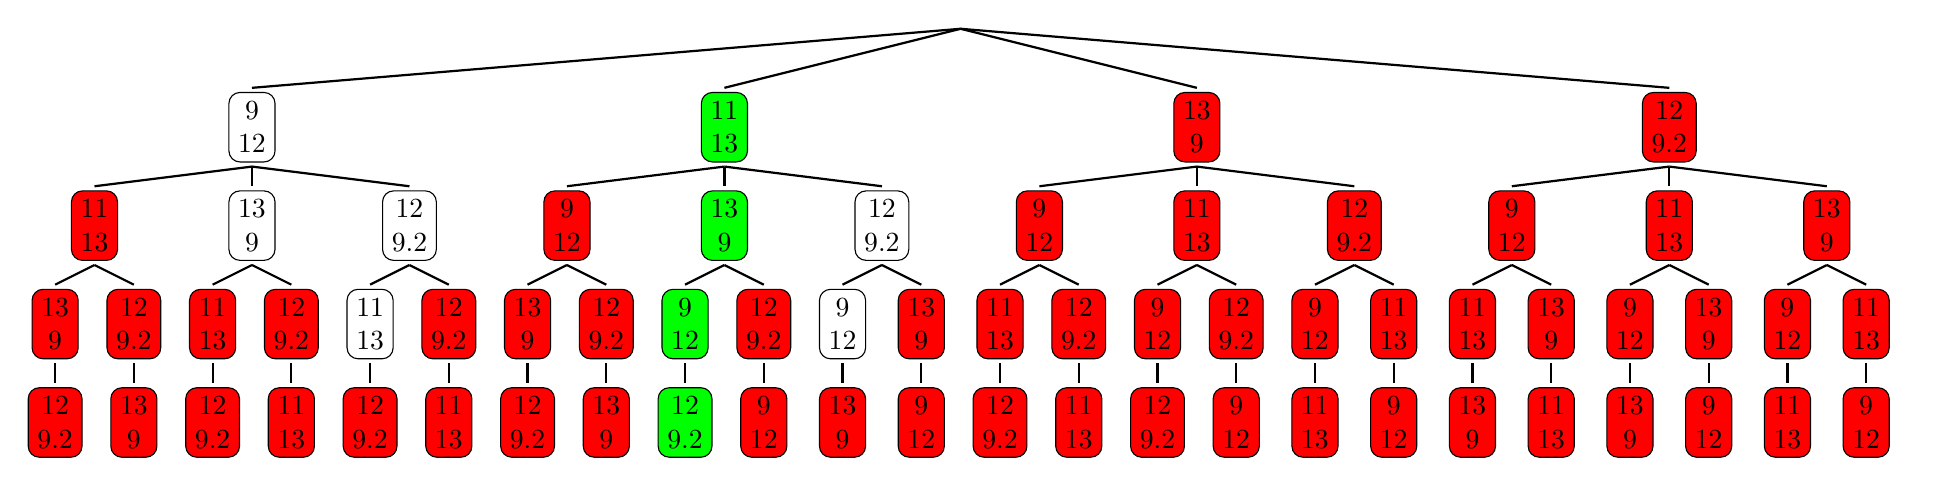
\begin{tikzpicture} [scale=.5]

		% level 4 lines
		\draw [thick] (24,10) -- (6,8.5);
		\draw [thick] (24,10) -- (18,8.5);
		\draw [thick] (24,10) -- (30,8.5);
		\draw [thick] (24,10) -- (42,8.5);

		% level 3 lines
		\draw [thick] (6,6.5) -- (2,6);
		\draw [thick] (6,6.5) -- (6,6);
		\draw [thick] (6,6.5) -- (10,6);
		\draw [thick] (18,6.5) -- (14,6);
		\draw [thick] (18,6.5) -- (18,6);
		\draw [thick] (18,6.5) -- (22,6);
		\draw [thick] (30,6.5) -- (26,6);
		\draw [thick] (30,6.5) -- (30,6);
		\draw [thick] (30,6.5) -- (34,6);
		\draw [thick] (42,6.5) -- (38,6);
		\draw [thick] (42,6.5) -- (42,6);
		\draw [thick] (42,6.5) -- (46,6);

		% level 2 lines
		\draw [thick] (2,4) -- (1,3.5);
		\draw [thick] (2,4) -- (3,3.5);
		\draw [thick] (6,4) -- (5,3.5);
		\draw [thick] (6,4) -- (7,3.5);
		\draw [thick] (10,4) -- (9,3.5);
		\draw [thick] (10,4) -- (11,3.5);
		\draw [thick] (14,4) -- (13,3.5);
		\draw [thick] (14,4) -- (15,3.5);
		\draw [thick] (18,4) -- (17,3.5);
		\draw [thick] (18,4) -- (19,3.5);
		\draw [thick] (22,4) -- (21,3.5);
		\draw [thick] (22,4) -- (23,3.5);
		\draw [thick] (26,4) -- (25,3.5);
		\draw [thick] (26,4) -- (27,3.5);
		\draw [thick] (30,4) -- (29,3.5);
		\draw [thick] (30,4) -- (31,3.5);
		\draw [thick] (34,4) -- (33,3.5);
		\draw [thick] (34,4) -- (35,3.5);
		\draw [thick] (38,4) -- (37,3.5);
		\draw [thick] (38,4) -- (39,3.5);
		\draw [thick] (42,4) -- (41,3.5);
		\draw [thick] (42,4) -- (43,3.5);
		\draw [thick] (46,4) -- (45,3.5);
		\draw [thick] (46,4) -- (47,3.5);

		% level 1 lines
		\draw [thick] (1,1.5) -- (1,1);
		\draw [thick] (3,1.5) -- (3,1);
		\draw [thick] (5,1.5) -- (5,1);
		\draw [thick] (7,1.5) -- (7,1);
		\draw [thick] (9,1.5) -- (9,1);
		\draw [thick] (11,1.5) -- (11,1);
		\draw [thick] (13,1.5) -- (13,1);
		\draw [thick] (15,1.5) -- (15,1);
		\draw [thick] (17,1.5) -- (17,1);
		\draw [thick] (19,1.5) -- (19,1);
		\draw [thick] (21,1.5) -- (21,1);
		\draw [thick] (23,1.5) -- (23,1);
		\draw [thick] (25,1.5) -- (25,1);
		\draw [thick] (27,1.5) -- (27,1);
		\draw [thick] (29,1.5) -- (29,1);
		\draw [thick] (31,1.5) -- (31,1);
		\draw [thick] (33,1.5) -- (33,1);
		\draw [thick] (35,1.5) -- (35,1);
		\draw [thick] (37,1.5) -- (37,1);
		\draw [thick] (39,1.5) -- (39,1);
		\draw [thick] (41,1.5) -- (41,1);
		\draw [thick] (43,1.5) -- (43,1);
		\draw [thick] (45,1.5) -- (45,1);
		\draw [thick] (47,1.5) -- (47,1);

		% level 4
		\node[align=center, rounded corners, draw, fill = white] at (6,7.5) {9\\12};
		\node[align=center, rounded corners, draw, fill = green] at (18,7.5) {11\\13};
		\node[align=center, rounded corners, draw, fill = red] at (30,7.5) {13\\9};
		\node[align=center, rounded corners, draw, fill = red] at (42,7.5) {12\\9.2};

		% level 3
		\node[align=center, rounded corners, draw, fill = red] at (2,5) {11\\13};
		\node[align=center, rounded corners, draw, fill = white] at (6,5) {13\\9};
		\node[align=center, rounded corners, draw, fill = white] at (10,5) {12\\9.2};
		\node[align=center, rounded corners, draw, fill = red] at (14,5) {9\\12};
		\node[align=center, rounded corners, draw, fill = green] at (18,5) {13\\9};
		\node[align=center, rounded corners, draw, fill = white] at (22,5) {12\\9.2};
		\node[align=center, rounded corners, draw, fill = red] at (26,5) {9\\12};
		\node[align=center, rounded corners, draw, fill = red] at (30,5) {11\\13};
		\node[align=center, rounded corners, draw, fill = red] at (34,5) {12\\9.2};
		\node[align=center, rounded corners, draw, fill = red] at (38,5) {9\\12};
		\node[align=center, rounded corners, draw, fill = red] at (42,5) {11\\13};
		\node[align=center, rounded corners, draw, fill = red] at (46,5) {13\\9};

		% level 2
		\node[align=center, rounded corners, draw, fill = red] at (1,2.5) {13\\9};
		\node[align=center, rounded corners, draw, fill = red] at (3,2.5) {12\\9.2};
		\node[align=center, rounded corners, draw, fill = red] at (5,2.5) {11\\13};
		\node[align=center, rounded corners, draw, fill = red] at (7,2.5) {12\\9.2};
		\node[align=center, rounded corners, draw, fill = white] at (9,2.5) {11\\13};
		\node[align=center, rounded corners, draw, fill = red] at (11,2.5) {12\\9.2};
		\node[align=center, rounded corners, draw, fill = red] at (13,2.5) {13\\9};
		\node[align=center, rounded corners, draw, fill = red] at (15,2.5) {12\\9.2};
		\node[align=center, rounded corners, draw, fill = green] at (17,2.5) {9\\12};
		\node[align=center, rounded corners, draw, fill = red] at (19,2.5) {12\\9.2};
		\node[align=center, rounded corners, draw, fill = white] at (21,2.5) {9\\12};
		\node[align=center, rounded corners, draw, fill = red] at (23,2.5) {13\\9};
		\node[align=center, rounded corners, draw, fill = red] at (25,2.5) {11\\13};
		\node[align=center, rounded corners, draw, fill = red] at (27,2.5) {12\\9.2};
		\node[align=center, rounded corners, draw, fill = red] at (29,2.5) {9\\12};
		\node[align=center, rounded corners, draw, fill = red] at (31,2.5) {12\\9.2};
		\node[align=center, rounded corners, draw, fill = red] at (33,2.5) {9\\12};
		\node[align=center, rounded corners, draw, fill = red] at (35,2.5) {11\\13};
		\node[align=center, rounded corners, draw, fill = red] at (37,2.5) {11\\13};
		\node[align=center, rounded corners, draw, fill = red] at (39,2.5) {13\\9};
		\node[align=center, rounded corners, draw, fill = red] at (41,2.5) {9\\12};
		\node[align=center, rounded corners, draw, fill = red] at (43,2.5) {13\\9};
		\node[align=center, rounded corners, draw, fill = red] at (45,2.5) {9\\12};
		\node[align=center, rounded corners, draw, fill = red] at (47,2.5) {11\\13};

		% bottom row (level 1)
		\node[align=center, rounded corners, draw, fill = red] at (1,0) {12\\9.2};
		\node[align=center, rounded corners, draw, fill = red] at (3,0) {13\\9};
		\node[align=center, rounded corners, draw, fill = red] at (5,0) {12\\9.2};
		\node[align=center, rounded corners, draw, fill = red] at (7,0) {11\\13};
		\node[align=center, rounded corners, draw, fill = red] at (9,0) {12\\9.2};
		\node[align=center, rounded corners, draw, fill = red] at (11,0) {11\\13};
		\node[align=center, rounded corners, draw, fill = red] at (13,0) {12\\9.2};
		\node[align=center, rounded corners, draw, fill = red] at (15,0) {13\\9};
		\node[align=center, rounded corners, draw, fill = green] at (17,0) {12\\9.2};
		\node[align=center, rounded corners, draw, fill = red] at (19,0) {9\\12};
		\node[align=center, rounded corners, draw, fill = red] at (21,0) {13\\9};
		\node[align=center, rounded corners, draw, fill = red] at (23,0) {9\\12};
		\node[align=center, rounded corners, draw, fill = red] at (25,0) {12\\9.2};
		\node[align=center, rounded corners, draw, fill = red] at (27,0) {11\\13};
		\node[align=center, rounded corners, draw, fill = red] at (29,0) {12\\9.2};
		\node[align=center, rounded corners, draw, fill = red] at (31,0) {9\\12};
		\node[align=center, rounded corners, draw, fill = red] at (33,0) {11\\13};
		\node[align=center, rounded corners, draw, fill = red] at (35,0) {9\\12};
		\node[align=center, rounded corners, draw, fill = red] at (37,0) {13\\9};
		\node[align=center, rounded corners, draw, fill = red] at (39,0) {11\\13};
		\node[align=center, rounded corners, draw, fill = red] at (41,0) {13\\9};
		\node[align=center, rounded corners, draw, fill = red] at (43,0) {9\\12};
		\node[align=center, rounded corners, draw, fill = red] at (45,0) {11\\13};
		\node[align=center, rounded corners, draw, fill = red] at (47,0) {9\\12};
		\node at (47.75,0) {};

	\end{tikzpicture}
\endpgfgraphicnamed
\end{document}